

M-tree also known as the Metric tree is a tree data structure constructed using a metric distance measure and relies on the triangle inequality for efficient range search queries. Similar to all other tree data structures, an M-tree data structure also has Leaf Nodes and non- Leaf nodes. Every non leaf node has a pointer to its parent node, a pointer to its subtree, its object information and a covering radius denoting maximum distance of a node to any node in its subtree.Every leaf node keeps a pointer to its parent and object information.\\

The M-tree data structure compartments the objects into nodes, which define regions of the metric space. The maximum capacity of the M-tree is M. For each database object to be indexed, there is an entry $O_j = [ O_j, id(O_j), dist(O_j , P(O_j )) ]$
in some leaf node.  $O_j$ stores the object information, mainly the data point feature values or dimension coordinates, id($O_j$) stores the id of the object and $dist(O_j , P(O_j ))$ stores the distance of it to its parent object. \\

A non-leaf node $O_r$ stores an object information as well as a covering radius $r(O_r)$ and a pointer to a subtree i.e. entry $O_r=[ O_r, ptr(T(O_r)), r(O_r), d(O_r, P(O_r)) ]$. One property satisfied is that every object $O_j$ stored in a subtree rooted at router object $O_r$ is at atmost $r(O_r)$ distance to it $d(O_j , O_r) ≤ r(O_r)$. M-tree organizes the metric space into a set of, possibly overlapping, regions, to which the same principle is recursively applied.\\


\section{Information in the data structure}

We use a modified data structure similar to the M-tree.We keep the following information in each node of the our modified M-tree: the object identifier of the pivot, i.e fingerprint information of the pivot fingerprint; the pivot also stores a pointer to its children i.e a pointer to a set of fingerprints; a double value which is the distance of the farthest child in its subtree and a boolean value which signifies if the pivot is an outlier pivot. We do not require a parent pointer. And the size of each node is determined by the number of pivots chosen at each step of our indexing technique and the base outlier size limit, which are explained later. The following information is stored in each entry of a node in our tree:

\begin{enumerate}
	\item Object identifier $p_i$
	\item Pointer to subtree $S_i$
	\item Farthest child i.e. Covering radius $r_i$
	\item Outlier pivot boolean variable
\end{enumerate}

\section{Baseline Indexing approach}
In the baseline approach, we are partitioning the dataset into groups using pivots which enables us to exploit the triangle inequality. The choice of pivots in the baseline approach is done randomly. The number of pivots is determined by two input parameters viz. the number of random pivots chosen at each step and the minimum size of the outlier set allowed at the lowest level. This has been formally explained in the algorithm below. \\

\begin{figure}[ht]	
\centering
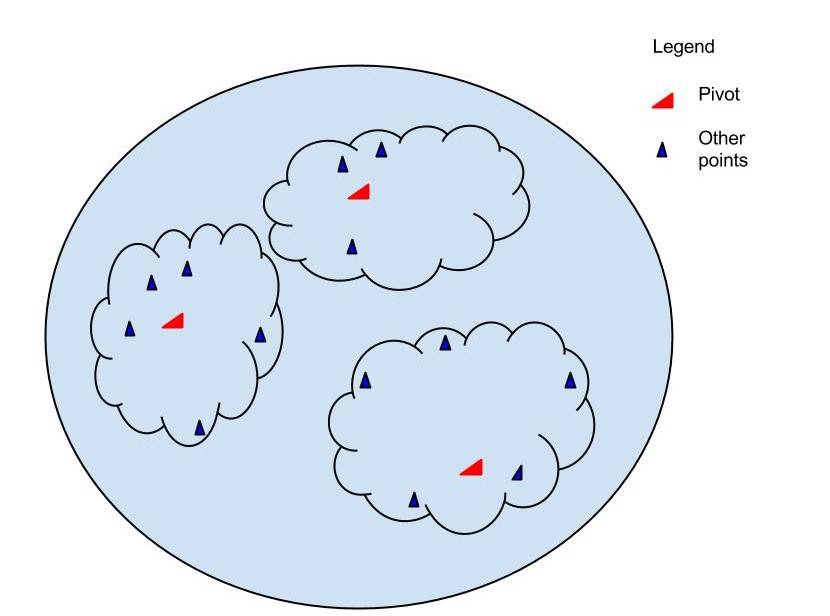
\includegraphics[width=0.7 \columnwidth]{img/image0a.jpg}
\caption{Assigning points to a cluster after the pivoting step of the M-tree indexing process}
\label{fig:4.1}
\end{figure}

\begin{figure}[ht]	
\centering
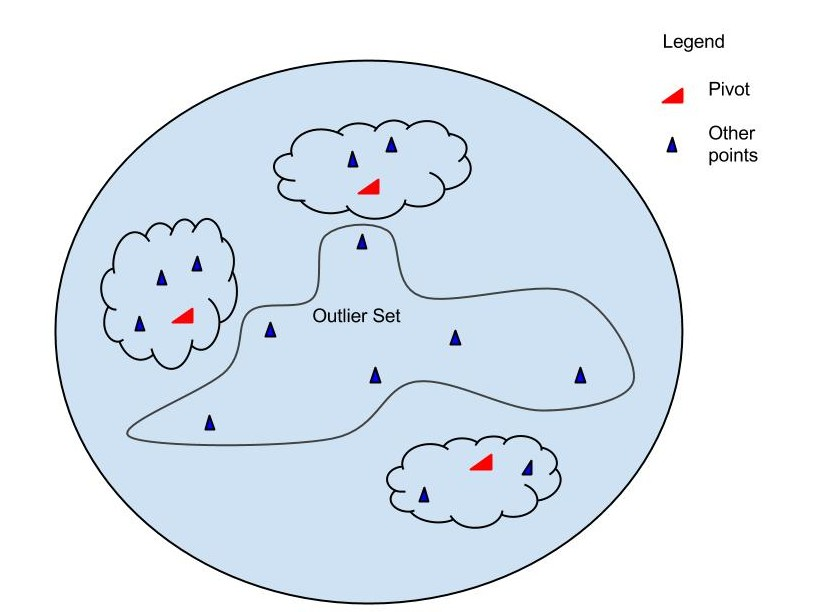
\includegraphics[width=0.7 \columnwidth]{img/image0b.jpg}
\caption{Finding the outlier set in the M-tree index structure}
\label{fig:4.2}
\end{figure}
\begin{enumerate}

\item Choose the given number of random pivots from the set. The number of random pivots chosen at this step is a parameter to our experiment and has been varied across different values.

\item After choosing pivots we assign every other chemical compound in the database to one of the pivots based on the similarity to the pivots. A chemical compound is assigned to the pivot which is nearest in distance to it i.e. it has the highest Min-Max similarity with that as compared to other pivots . This is described in \autoref{fig:4.1}.

\item The next step involves ranking all chemical compounds data points by their similarity to their own closest pivot. 

\item We calculate the median similarity among all the chemical compounds in this database and note it as the outlier cut-off/

\item All the chemical compounds with similarity less than the cut-off similarity is called as outliers in this step

\item The outliers are unassigned from the pivots and assigned to the "outlier" pivot. This has been described in \autoref{fig:4.2}

\item We recursively apply this technique on the outlier set until the outlier set size reaches a base limit which is also a parameter to our algorithm.\\

\end{enumerate}


\section{Alternate indexing approach}

We tried an alternate approach where instead of choosing outliers after assigning molecules the most similar pivot we recursively apply the technique on each set. In simpler words, we try to cluster at each step and try to create clusters among each cluster recursively. So in each cluster we choose pivots again and try to assign each of the points to the pivots until we cannot choose more pivots. We can formally explain it as follows.


\begin{enumerate}

\item Choose the given number of random pivots from the set. The number of random pivots chosen at this step is again a parameter to the experiment as previously.

\item The second step is also similar to the earlier indexing technique. After choosing pivots we assign every other chemical compound in the database to one of the pivots based on the similarity to the pivots.
 
\item Instead of choosing outliers now, we work with the same sets and recursively apply this technique on the set until the set size reaches a base limit .

\item The set size limit is set as the number of pivots chosen at each step i.e. the method is applied recursively on the set until the size of the set is lower than the pivot set size making us unable to choose pivots. \\

\end{enumerate}

The previous indexing technique was seen to give us better results. Hence we will be using the earlier technique for all experimental evaluations. One reason we could think of why this technique failed is probably because the tree was becoming more imbalanced and the height was increasing causing querying time to be more.



\section{Choosing pivot}

Instead of randomly choosing pivots at every step we use a Max-Min distance approach where we try to maximize the minimum distance between any two pivot nodes chosen. The procedure can be explained as below:

\begin{enumerate}
	\item Choose a random point.
	\item The second point chosen is such that it is farthest from the first chosen random point. This will require a full database scan
	\item The third point is chosen such that its minimum distance to either of the previous two pivots is maximized.
	\item Iteratively, the $i^{th}$ point is chosen in a fashion such that the minimum of its distance to the previous i-1 points is maximized.
	\item This procedure is repeated till we choose $p$ points where p is the number of pivots to be chosen	\\

\end{enumerate} 

We can observe that this is a very expensive procedure since we are scanning the entire database at every step. We need to compute an all pair similarity initially. At the $i^{th}$ step , the remaining n-i+1 points in  database need to compute its minimum distance to the i-1 points already present in pivot step. Finally choose the point among the n-i+1 points with the maximum distance. This computation is of the O($n^3$).
	\[T(n)=  n^2 + \sum \limits_{i=1}^{n}( (n-i+1)(i-1)  + n-i+1) \]
	\[T(n)=O(n^3)\]

We use a sampling technique where we randomly sample a subset of the database and apply the technique described above on the subset. We used a subset size of $\frac{1}{10^{th}}$ the size of the database, approximately about 20,000 points in the subset.


\begin{figure}[ht!]	
\centering
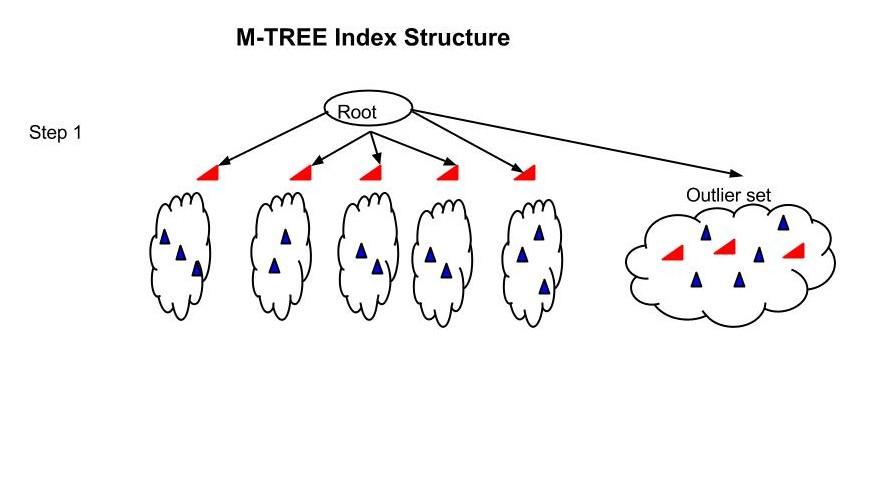
\includegraphics[width=1 \columnwidth]{img/image0d.jpg}
\caption{M-tree tree structure Step 1}
\label{fig: step1}
\end{figure}


\begin{figure}[ht!]	
\centering
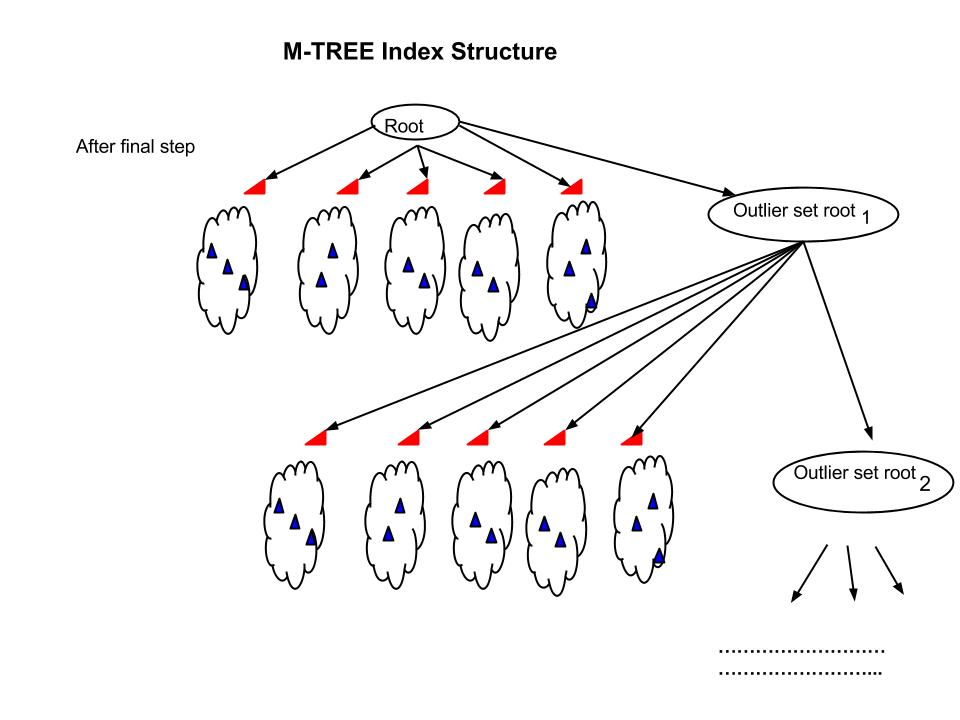
\includegraphics[width=1 \columnwidth]{img/image0e.jpg}
\caption{M-tree tree structure - After final step}
\label{fig: final step}
\end{figure}




\section{Range Search Querying}

Given a query chemical fingerprint $q$ and a threshold $\theta $ we want to find the set of chemical fingerprints which satisfy the query. We exploit the triangle inequality for the same. The procedure for range search querying can be described by the following steps\\

\begin{enumerate}
	\item The basic idea is to be able to prune subtrees based on the covering radius of the pivot of the subtree and the distance of the query to the pivot
	 
	\item Let the query fingerprint be q and the fingerprint pivot be $p_i$ of subtree $S_i$. We can calculate the maximum distance of any node in $S_i$ from q.We start with the root of the tree as $p_i$
	
	\item Let the covering radius of pivot $p_i$ be $r_i$. Hence the maximum distance of any node in $S_i$ will be $dist(q,p_i)$ + $r_i$. Similarly the minimum distance of any node in $S_i$ is $max(dist(q,p_i)$ - $r_i, 0)$. 
	
	\item Hence we can calculate the range of the distance of any node in $S_i$ to q. 
	
	\item  If the upper bound of the range or the maximum distance is lesser than the threshold distance $\theta$ we can add all the nodes in $S_i$ to our resultant set
	
	\item If the lower bound of the range is greater than the threshold distance $\theta$, we can prune the subtree $S_i$ since we can say with certainty that the distance of every node in the subtree $S_i$ is greater than  the threshold $\theta$.
	
	\item If there is an intersection in the intervals we recursively apply this technique on the second level of children in the subtree $S_i$ until we reach a leaf node.
	
\end{enumerate}



\section{Lipschitz Embedding}

The performance of the M-tree is limited by the fact that the data is very sparse. This results in very loose clusters being formed during the indexing phase. To improve upon this we performed an embedding of the data into Euclidean space using Lipschitz embedding. Lipshcitz embedding results in a contractive mapping.\\

Lipschitz embedding is the embedding, or in simpler words, dimensionality reduction of the objects of
a database D with metric distance d onto a k-dimensional feature vector space. The procedure goes as follows:
\begin{enumerate}
	\item Choose k subsets of D
	\item Each subset $A_i$ is a reference set
	\item Let the distance of object $p_j$ to set $A_i$ be:
	\[ d(p_j,A_i)= min_{a\epsilon A_{i}}      d(p_j,a) \]
	\item The feature vector f(o) is then defined as:
	\[f(p_j)= {\frac{d(p_j,A_1)}{k},\frac{d(p_j,A_2)}{k}...\frac{d(p_j,A_k)}{k}} \]
	\item We define the new distance $d'(f(p_j),f(p_k))$ as :
	\[d'(f(p_j),f(p_k)) = \sum \limits_{i=1}^{k} | d(p_j,A_i)-d(p_k,A_i)|\] 
\end{enumerate}

	We chose the reference sets in our embedding procedure as singleton sets. The choice of these points is done such that they are maximally far apart, i.e., the average and minimum all pairs distance among the reference sets is maximized similar to the method of choosing pivots in our indexing technique. This criteria of selecting the sets was based on the heuristic that farthest point will be maximally representative of the dataset. Since choice of such an optimal set is NP-hard, we perform a randomized set construction.\\

\begin{enumerate}
	\item Choose a random pivot from a sampled set of  data set points

	\item Add the point to our Reference set

	\item Find the point farthest from the reference set from the sampled set of points

	\item Add the point to the reference set

	\item Repeat step 3-4 until Reference set is full\\
\end{enumerate}

The dimension of the embedded space for the Swamidass dataset was chosen to be 514, which is the square root of the total number of points in the data set.We then performed M-tree based indexing and searching on this dataset. Our performance had deteriorated from that of the baseline technique. In later section we shall give a reasoning for this deterioration.